\section{Applying LIME}

\nblink{nhs-chest-xray/analyze/lime.ipynb}


\begin{figure}[h]
\centering
\caption{Scan 0 LIME output}
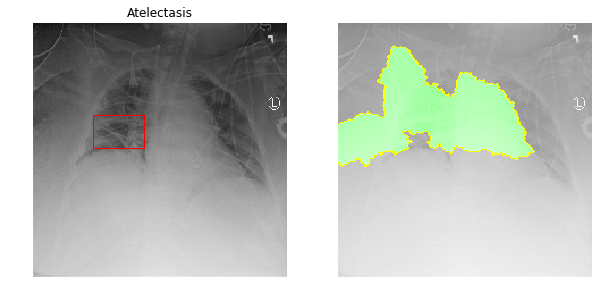
\includegraphics[width=12cm]{chapters/03_classification/images/lime_0.png}
\end{figure}

\begin{figure}[h]
\centering
\caption{Scan 2 LIME output}
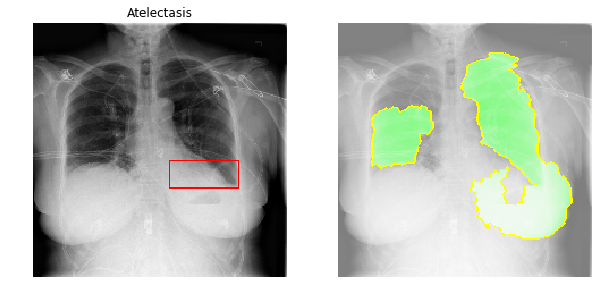
\includegraphics[width=12cm]{chapters/03_classification/images/lime_2.png}
\end{figure}

\begin{figure}[h]
\centering
\caption{Scan 8 LIME output}
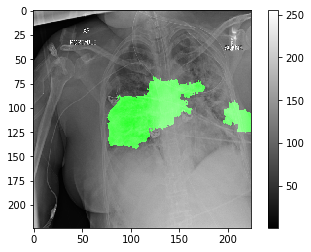
\includegraphics[width=12cm]{chapters/03_classification/images/lime_8.png}
\end{figure}

\subsection{LIME configuration}
\nblink{nhs-chest-xray/analyze/lime\_num\_features.ipynb}

\begin{figure}[h]
\centering
\caption{LIME Superpixel count: 1, 3, 6, 9}
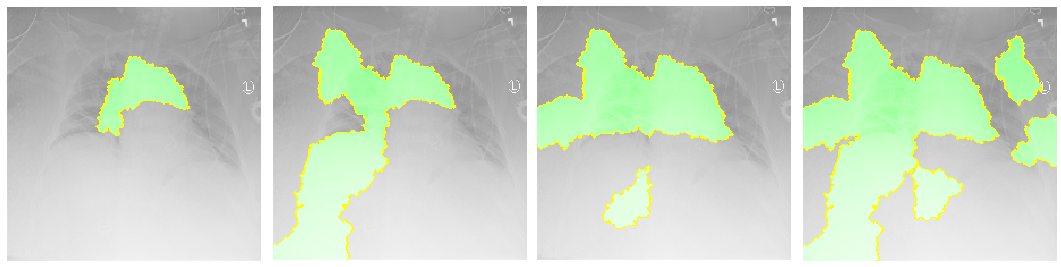
\includegraphics[width=14cm]{chapters/03_classification/images/lime-superpixel.png}
\end{figure}